
% ----------------------------------------------------------
% Apêndices
% ----------------------------------------------------------

% ---
% Inicia os apêndices
% ---
\begin{apendicesenv}

% Imprime uma página indicando o início dos apêndices
%\partapendices

\chapter{Aplicação do Questionário (CKAQ)}\label{chap:teste}

\noindent
\textbf{Instruções:}

O meu nome é \rule{3.0cm}{0.15mm} e eu preciso da sua ajuda para perceber o que as crianças da sua idade pensam sobre diferentes tipos de toques entre as pessoas. 

Voccê sabe que existem, pelo menos 3 tipos de toques diferentes? Às vezes você se sente bem quando alguém lhe toca – esses são os \underline{bons} toques – como os abraços ou algumas palmadinhas nas costas. Alguns toques são \underline{maus} - como os beliscões e dentadas, porque te deixam triste ou te fazem sentir desconfortável. Até alguns beijos de pessoas de quem  você não gosta podem ser maus toques. Às vezes alguns toques são \underline{confusos} – esses acontecem quando você não sabe dizer se são bons ou maus toques. Por exemplo, alguém de quem você gosta pode te dar um abraço, mas pode te apertar demais. É você quem deve decidir se um toque é bom ou mau, porque é você que sabe como é que esse toque faz você se sentir.

Outra palavra que eu quero ter a certeza que você entenda é: \underline{partes privadas}. Essas são as partes do seu corpo que são cobertas por uma roupa de praia. 

Vou lhe apresentar algumas questões sobre diferentes tipos de toques. Isto não é um teste escolar, você não será avaliado pelas suas respostas. Responda de acordo com o que você achar que está certo. Eu vou ler algumas perguntas e vou pedir para que responda “Sim” se achar que o que eu li é verdade, “Não” se achar que o que eu li é mentira e “Não sei” se não tem certeza se o que eu li é verdade ou mentira. 

\vspace{1.0cm}

\noindent
\textbf{NOTA:} Recomenda-se a administração verbal deste questionário para todas as crianças, especialmente se o CKAQ for usado para comparação entre crianças de diferentes idades em que as competências de leitura serão diferentes. Quando se lê os itens é importante acabarmos cada frase com ``\textbf{É verdade ou mentira?}''.

\vspace{1.0cm}

\begin{center}
	A aplicação deste questionário demora entre 10 a 15 minutos.
\end{center}


%-----------------------------------------------------------------------------------------------

\chapter{Children’s Knowledge of Abuse Questionnaire Revised – III  (Traduzido)}\label{chap:traduzido}

\noindent
\textbf{Identificação da Escola: \rule{2.0cm}{0.15mm} \quad Idade: \rule{1.2cm}{0.15mm} \quad Masculino \makebox[0pt][l]{$\square$}{} \quad  ou Feminino \makebox[0pt][l]{$\square$}{}}

\vspace{0.5cm}

\noindent
\textbf{Por favor responda V para ``Verdadeiro'', F para ``Falso'' e N para ``Não Sei'', para as seguintes questões: }

\begin{enumerate}
	\item Você sempre deve guardar segredos.
	\item Está tudo bem se alguém que você gosta lhe abraçar.
	\item Você sempre pode dizer quem é um estranho - pois eles parecem malvados.
	\item A maioria das crianças gostam de receber um beijo dos pais antes de ir para a cama à noite, então, para elas, isso seria um bom toque.
	\item Às vezes não há problemas em dizer ``não'' a um adulto.
	\item É normal dizer ``não'' e se afastar de alguém que tenha tocado em você de uma forma que você não gosta.
	\item Mesmo que alguém diga que te conhece, se você não o conhece, é um estranho.
	\item Mesmo os abraços e  as cócegas podem se transformar em toques ruins se durarem muito.
	\item Se você cair de sua bicicleta e machucar suas partes íntimas, não há problemas em um médico ou enfermeira examinar seu corpo.
	\item Se alguém lhe tocar de uma maneira que você não gosta, você deve contar sobre isso a alguém de sua confiança.
	\item Se o seu amigo disser que não será mais seu amigo se você não lhe der o último pedaço de bolo, então você deve dar a ele.
	\item Se alguém lhe tocar de uma maneira que você não gosta, é sua própria culpa.
	\item Se você não gosta de como alguém está tocando em você, não há problema em dizer ``não''.
	\item Estranhos parecem pessoas comuns.
	\item Se um adulto lhe diz para fazer algo, você sempre tem que fazer.
	\item Alguns toques começam bem, depois tornam-se confusos.
	\item Você pode confiar em seus sentimentos sobre se um toque é bom ou ruim.
	\item Tudo bem receber um abraço de um adulto de quem você gosta.
	\item Se um garoto malvado na escola manda você fazer algo, você deve fazer.
	\item Até mesmo alguém de quem você gosta pode tocá-lo de uma forma que faz você se sentir mal.
	\item Um tapinha nas costas de um professor de quem você gosta depois de ter feito um bom trabalho na escola é um bom toque.
	\item Você tem que deixar os adultos tocarem em você, goste ou não.
	\item Se alguém tocar em você de uma forma que não lhe faça bem, conte sobre isso até alguém acreditar em você.
	\item Às vezes, alguém da sua família pode tocar em você de uma maneira que você não goste.
	\item Os meninos não precisam se preocupar com alguém tocando suas partes íntimas.
	\item Se você está andando na rua com sua mãe e ela começa a conversar com um vizinho que você ainda não conhece, não há problema em conversar com ele.
	\item Se o pai de um amigo lhe pedir para ajudá-lo a encontrar um gatinho perdido, você deve ir imediatamente com ele e ajudá-lo.
	\item Se você ganhar um concurso da sua escola e um vizinho que você gosta lhe der um rápido abraço para parabenizá-lo, isso seria um bom toque.
	\item A maioria das pessoas são estranhas e a maioria dos estranhos é legal.
	\item Alguém que você conhece, mesmo um parente, pode querer tocar suas partes íntimas de uma forma que pareça confusa.
	\item Se sua babá diz para você tirar toda a roupa, mas não é hora de se despir para tomar banho, você tem que fazer isso.
	\item Se alguém entrar no banheiro enquanto você está tomando banho e você se sentir desconfortável, você deve ficar quieto.
	\item Se você se separar de seus pais em um local público, não há problemas em você pedir ajuda a um funcionário ou segurança, mesmo que sejam estranhos.
\end{enumerate}


%\null
%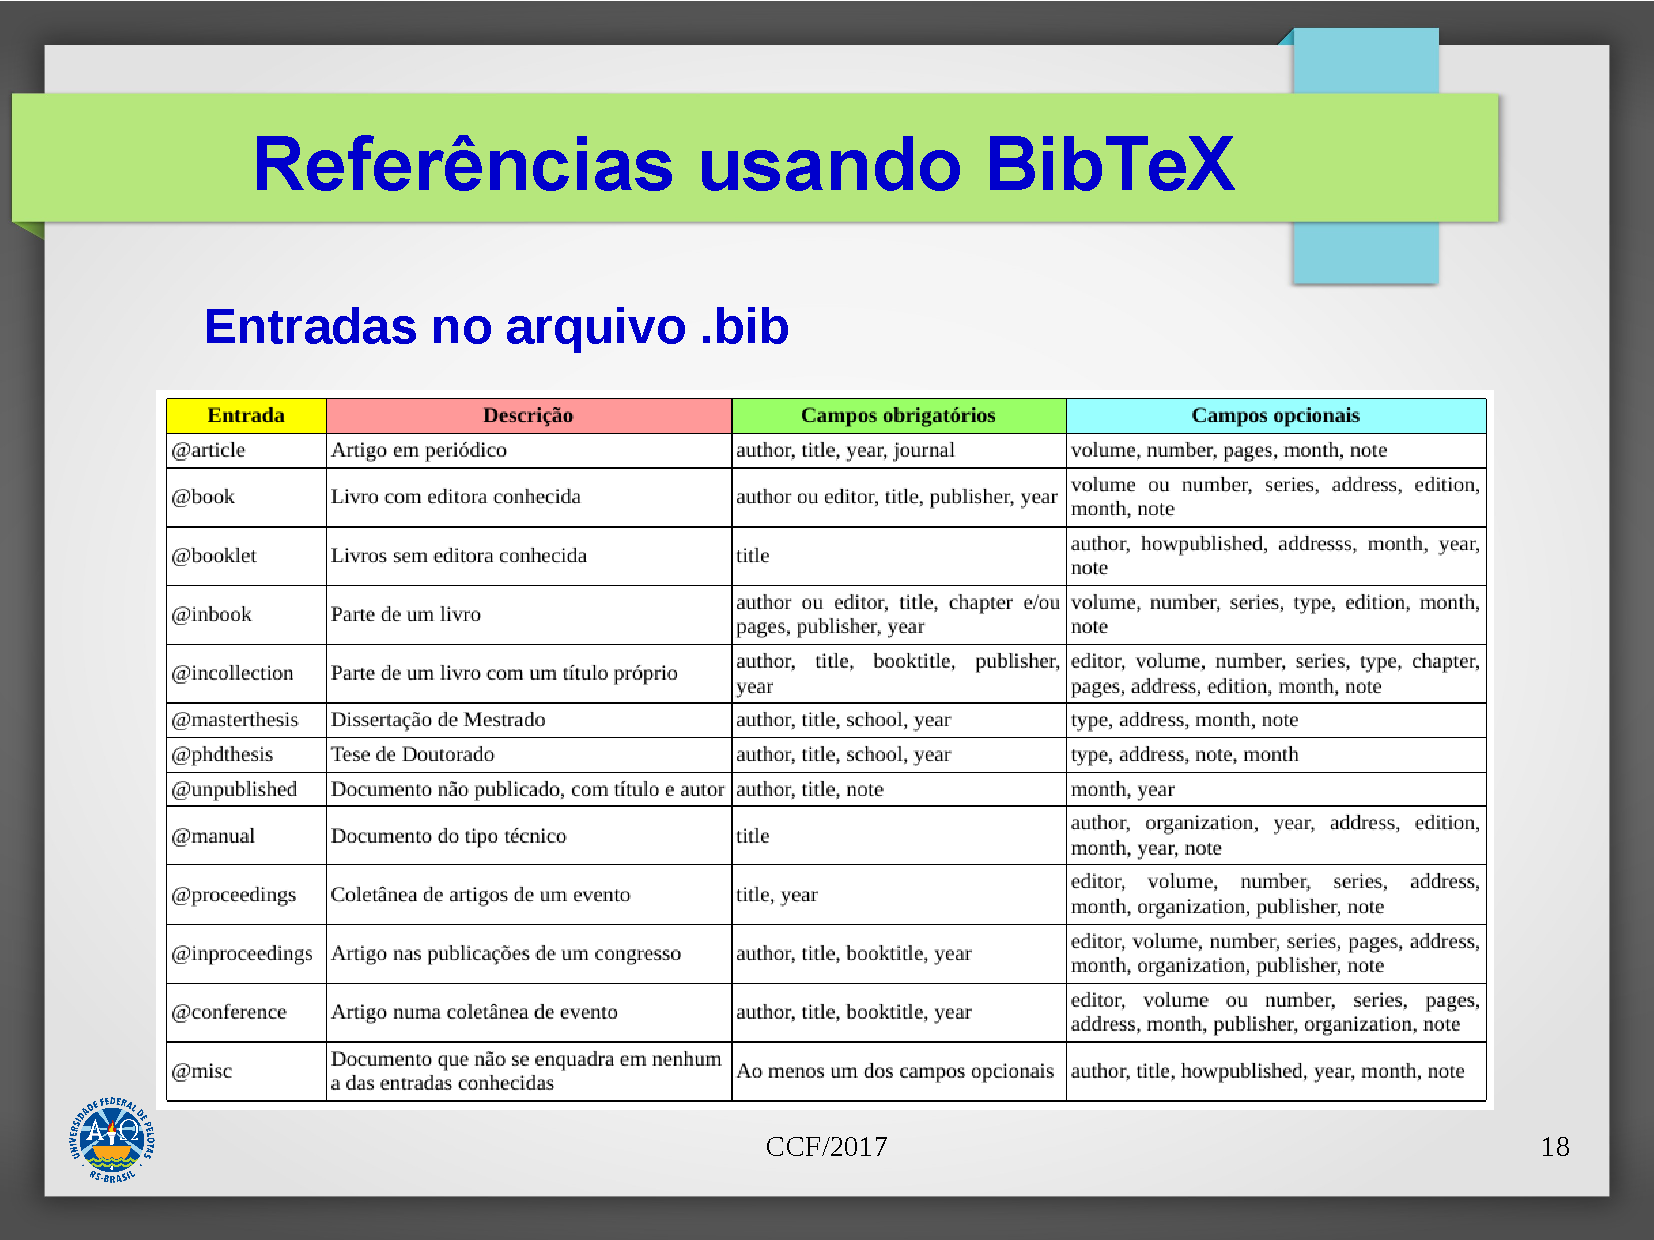
\includepdf[pages=-]{./Termos/a.pdf}

%-----------------------------------------------------------------------------------------------

\chapter{Declaração das Instituições Envolvidas}\label{chap:DIE}

\vspace{-1.5cm}\hspace{-3.0cm}\frame{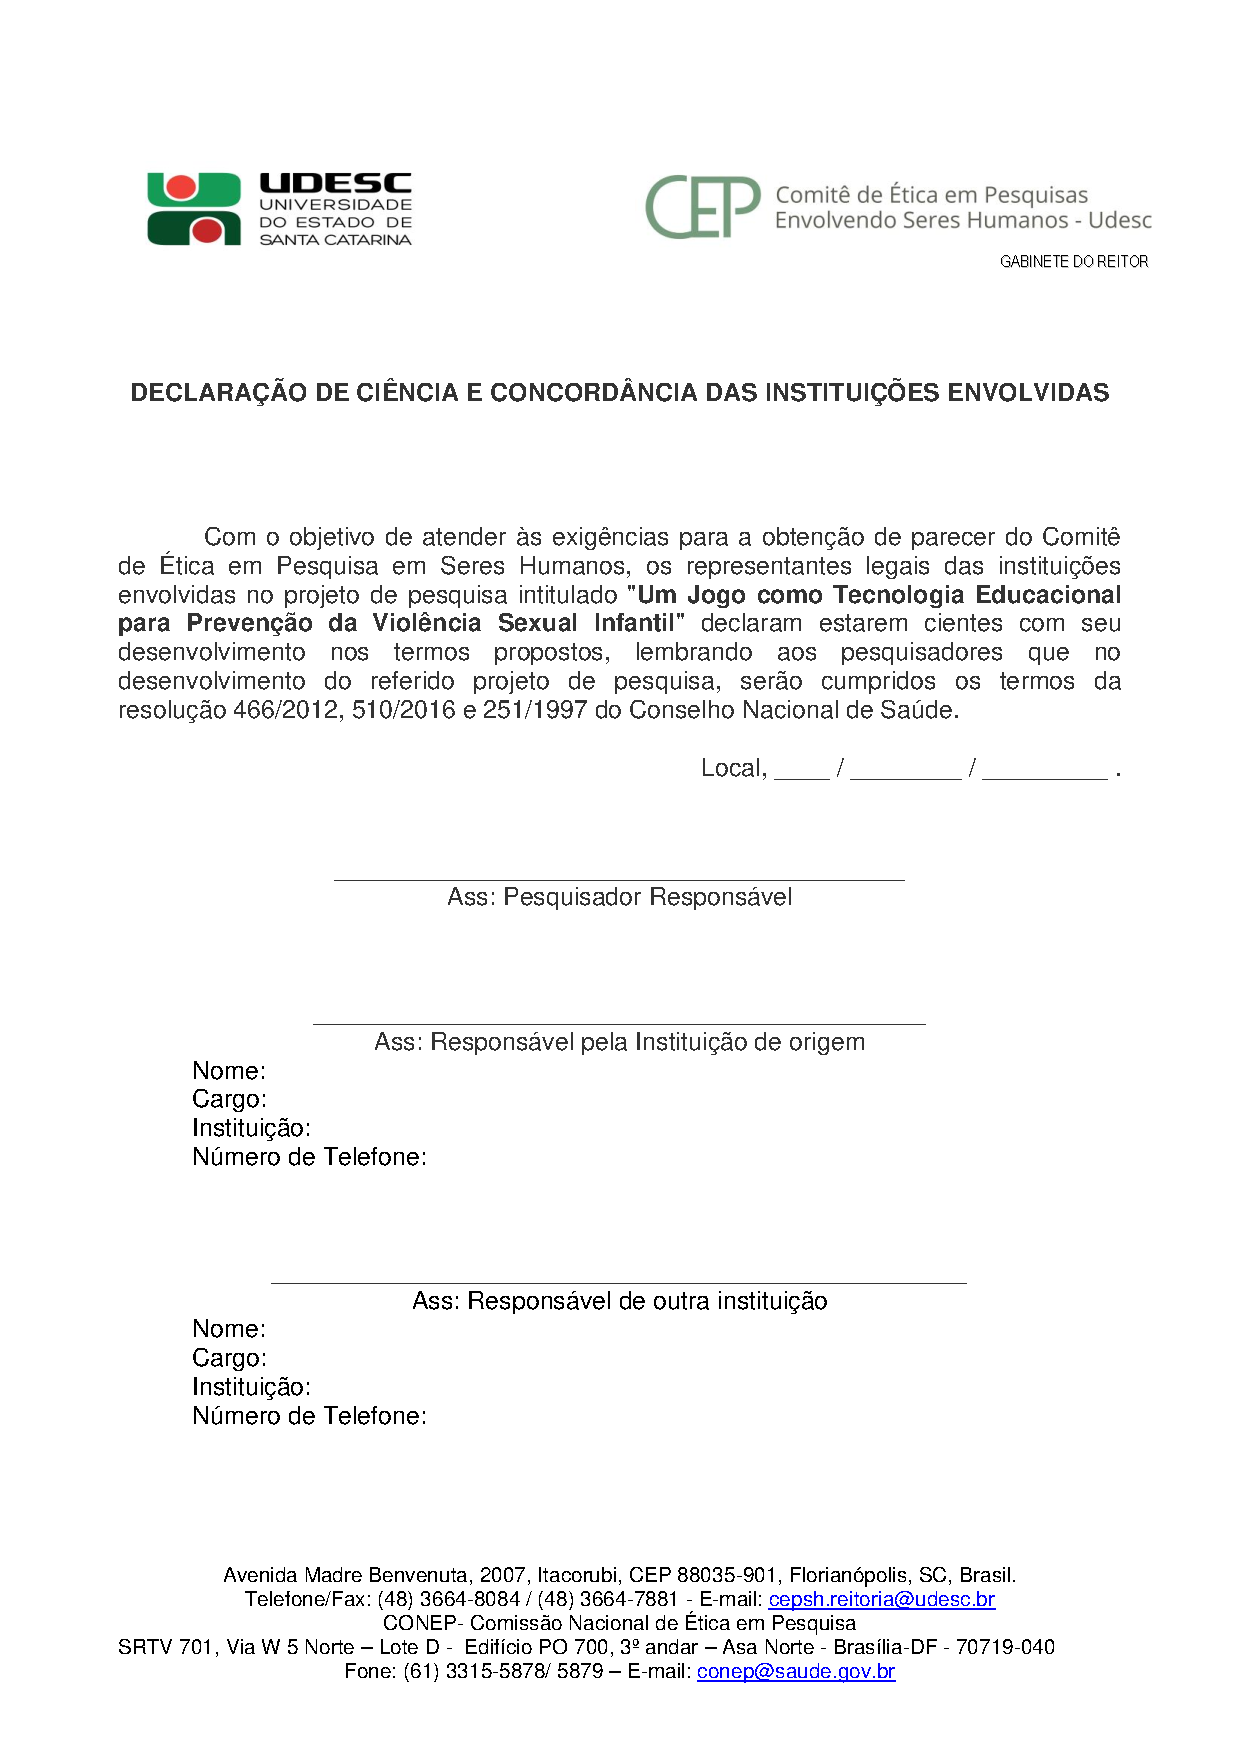
\includegraphics[scale=0.9]{./Termos/[Adapatado] Declaração das Instituições Envolvidas.pdf}}


%-----------------------------------------------------------------------------------------------

\chapter{Termo de Assentimento}\label{chap:TA}

\vspace{-1.5cm}\hspace{-3.0cm}\frame{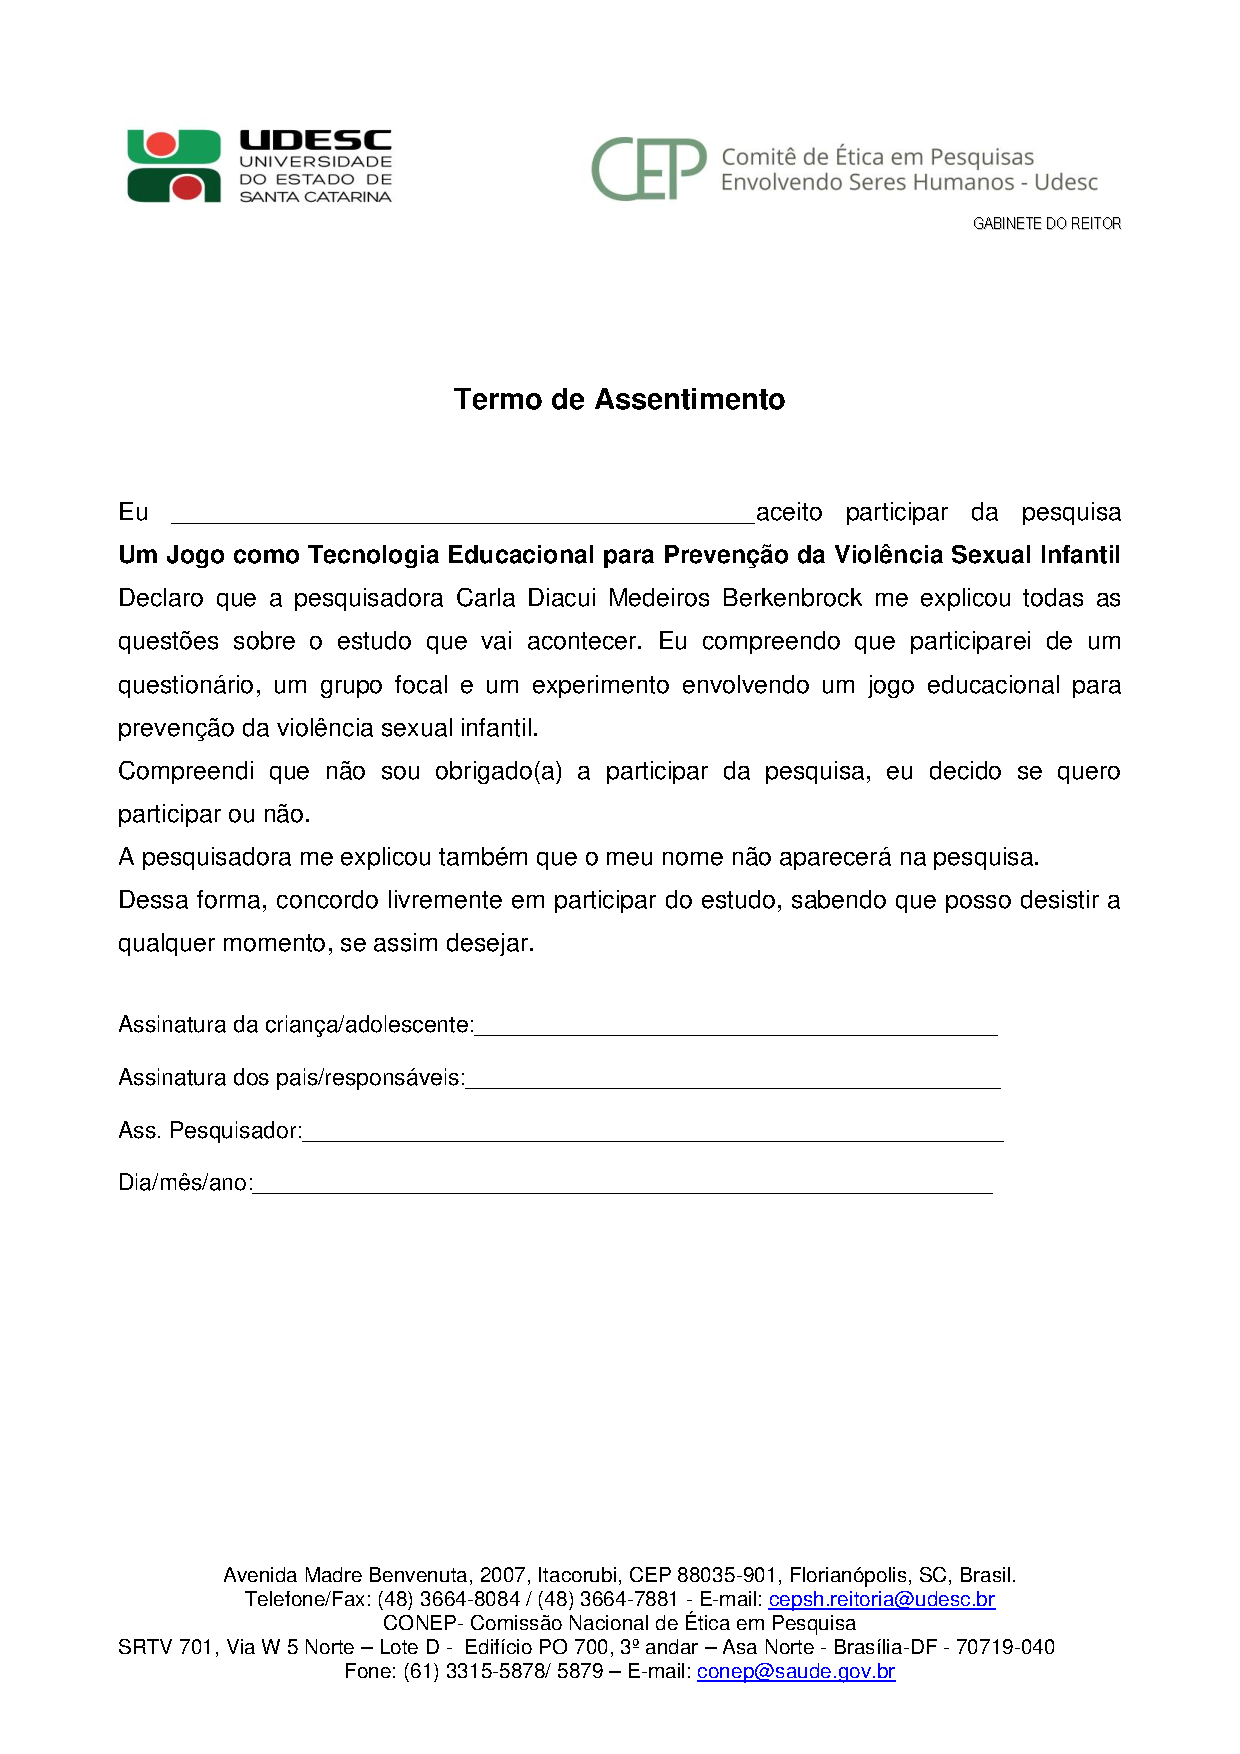
\includegraphics[scale=0.9]{./Termos/[Adaptado] Termo de Assentimento.pdf}}

%-----------------------------------------------------------------------------------------------

\chapter{Termo de Consentimento Livre e Esclarecido}\label{chap:TCLE}

\vspace{-1.5cm}\hspace{-3.0cm}\frame{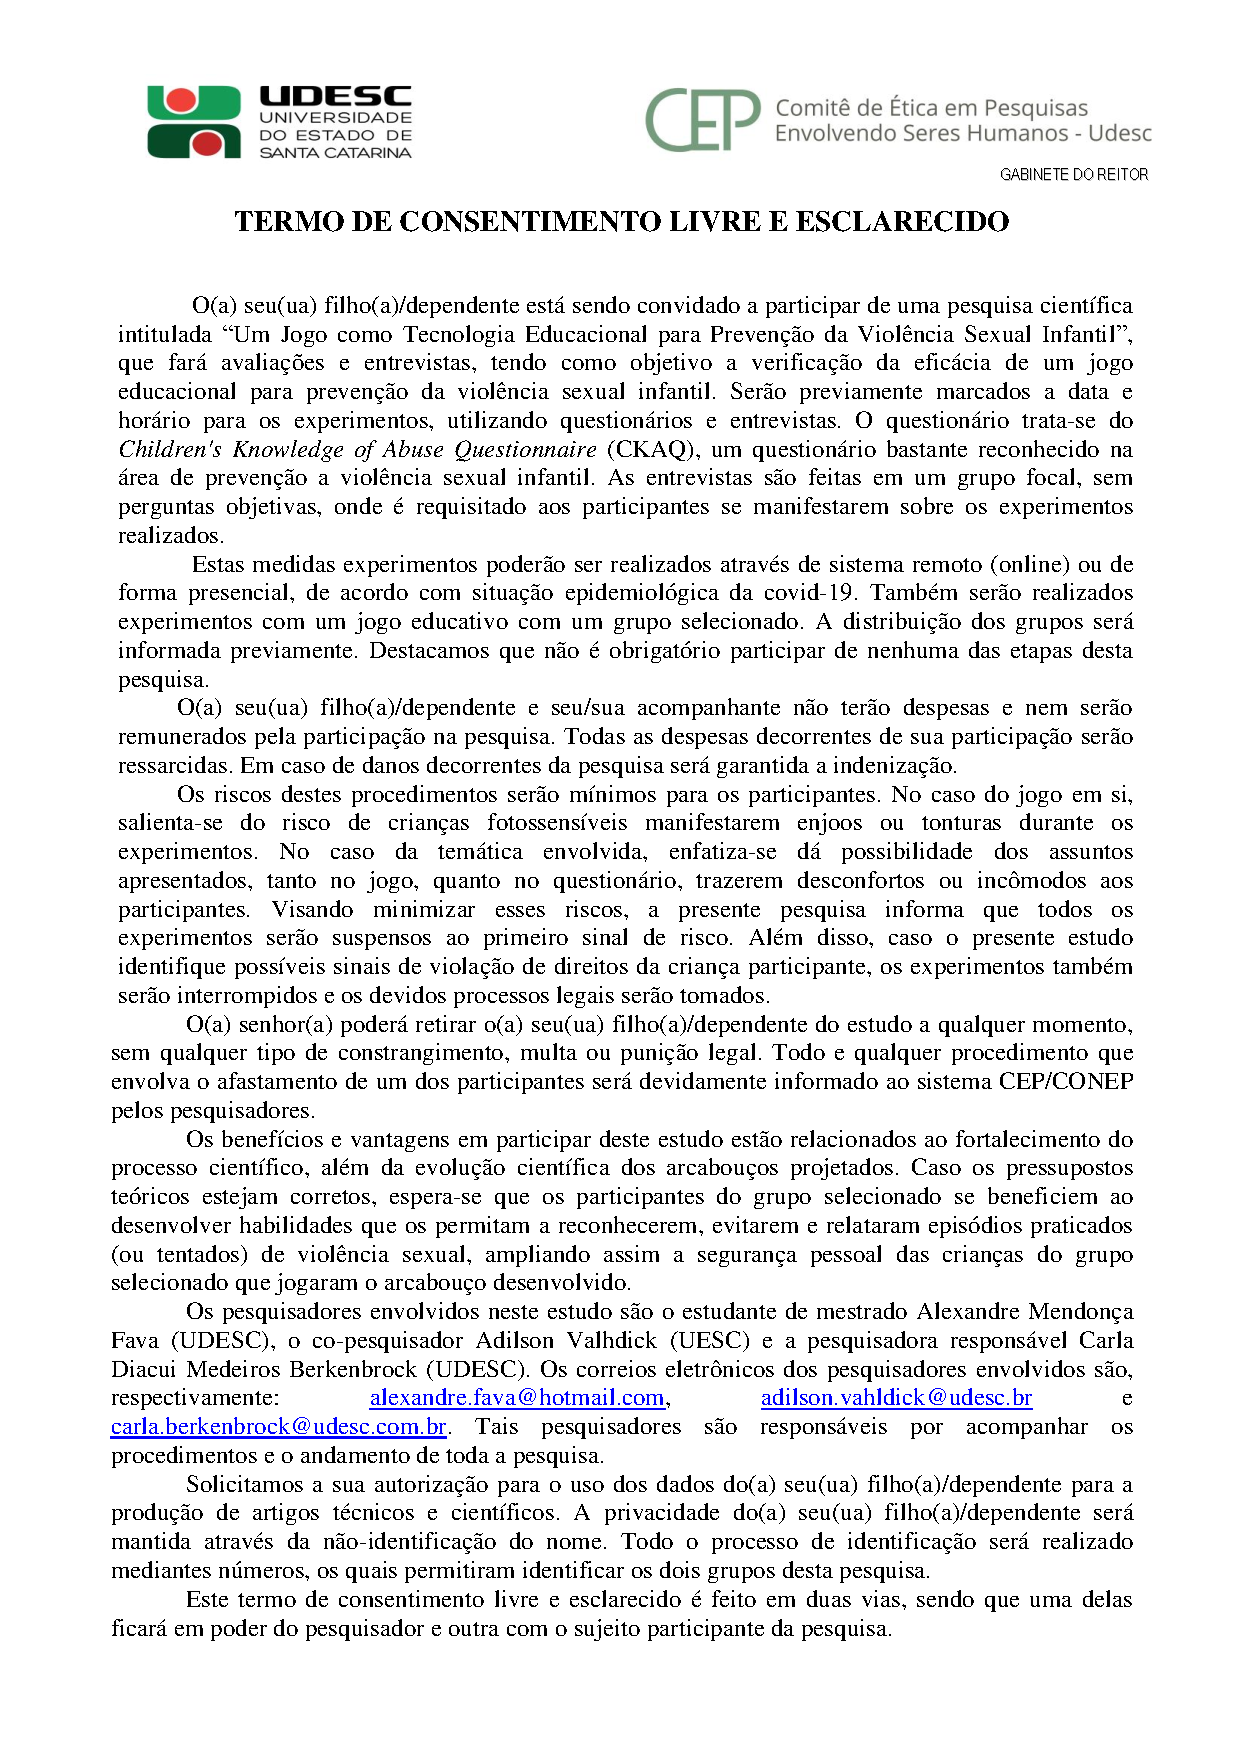
\includegraphics[scale=0.9]{./Termos/[Adaptado] Termo de Consentimento Livre e Esclarecido - Menores de Idade.pdf}}

%-----------------------------------------------------------------------------------------------

\chapter{Termo de Consentimento para Fotografias}\label{chap:TCF}

\vspace{-1.5cm}\hspace{-3.0cm}\frame{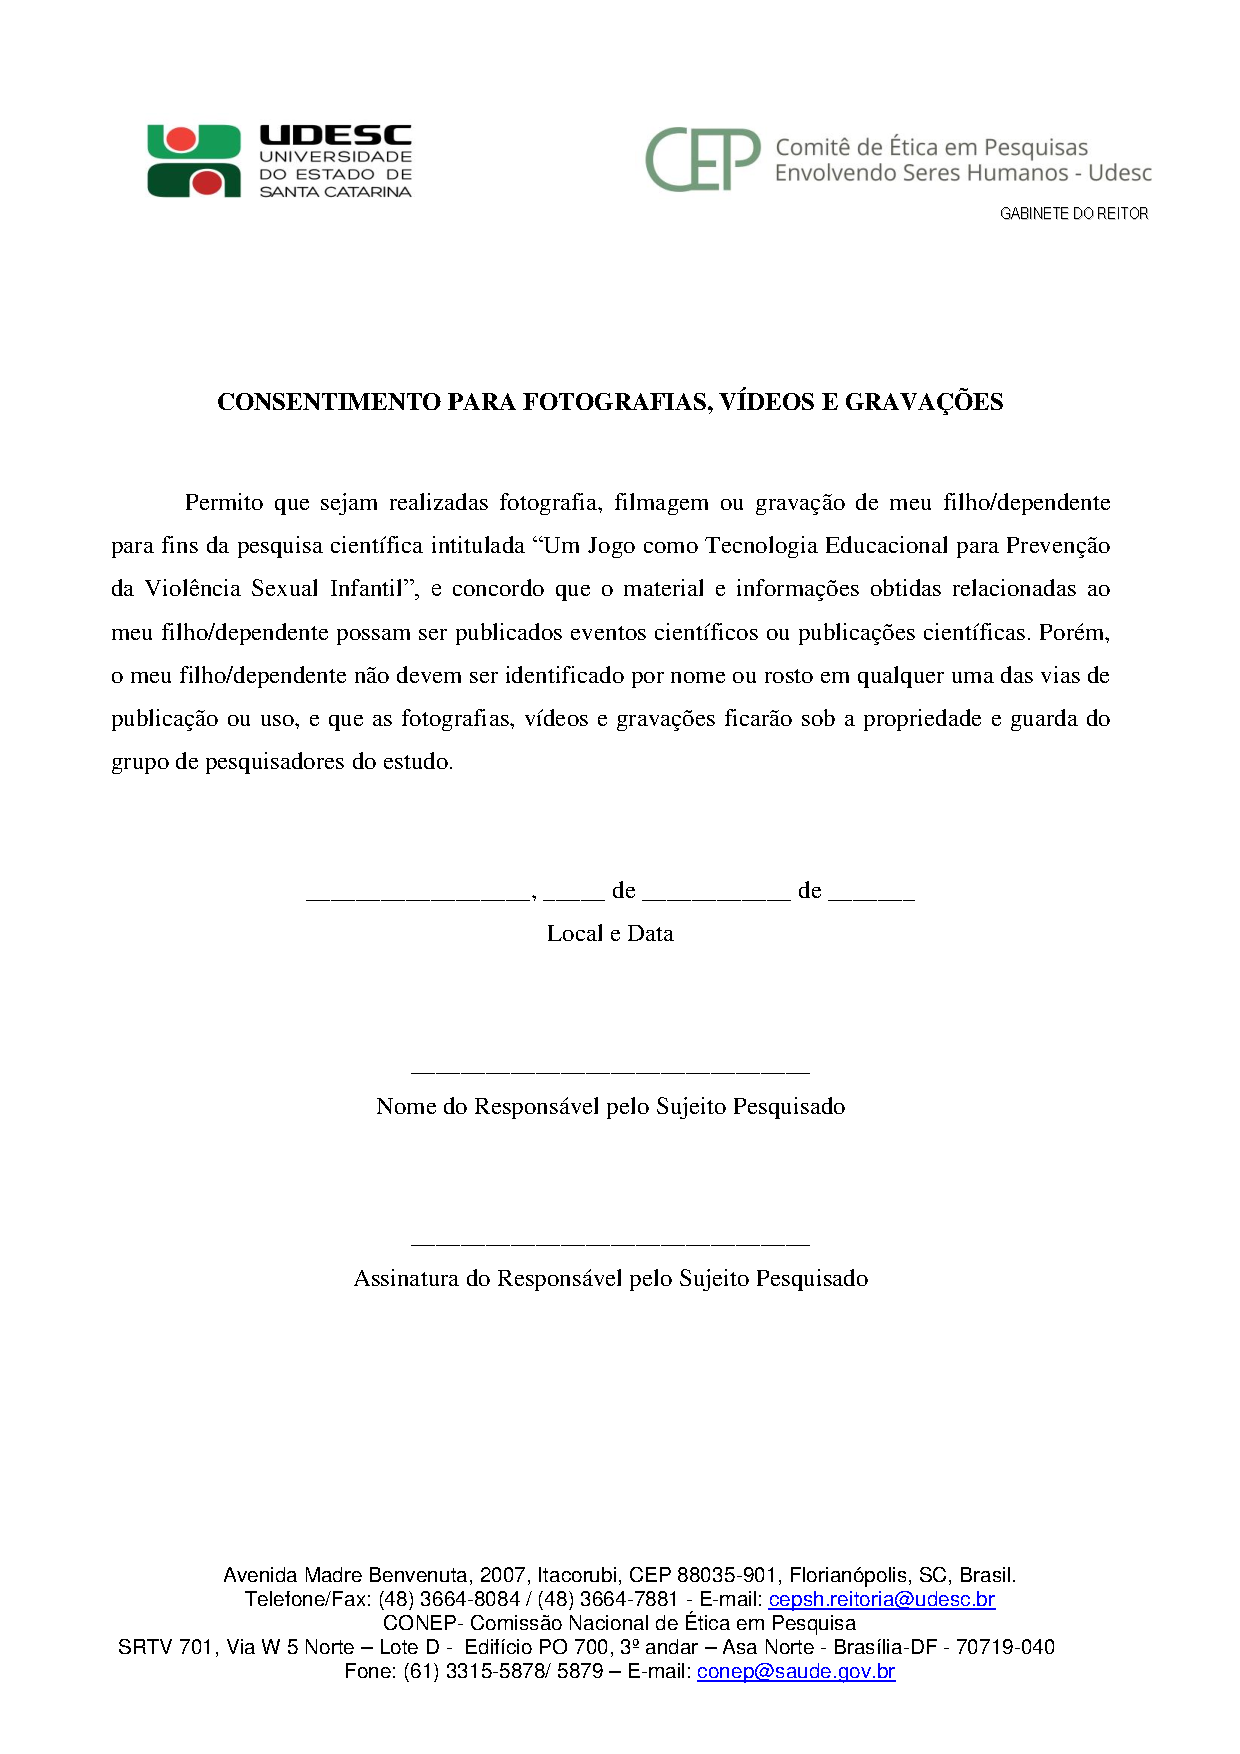
\includegraphics[scale=0.9]{./Termos/[Adaptado] Termo de Consentimento para Fotografias - Menores de Idade.pdf}}




\end{apendicesenv}
% ---